\documentclass[border=10pt]{standalone}
\usepackage{pgfplots}
\pgfplotsset{compat=1.18}
\usepgfplotslibrary{colormaps}

\begin{document}
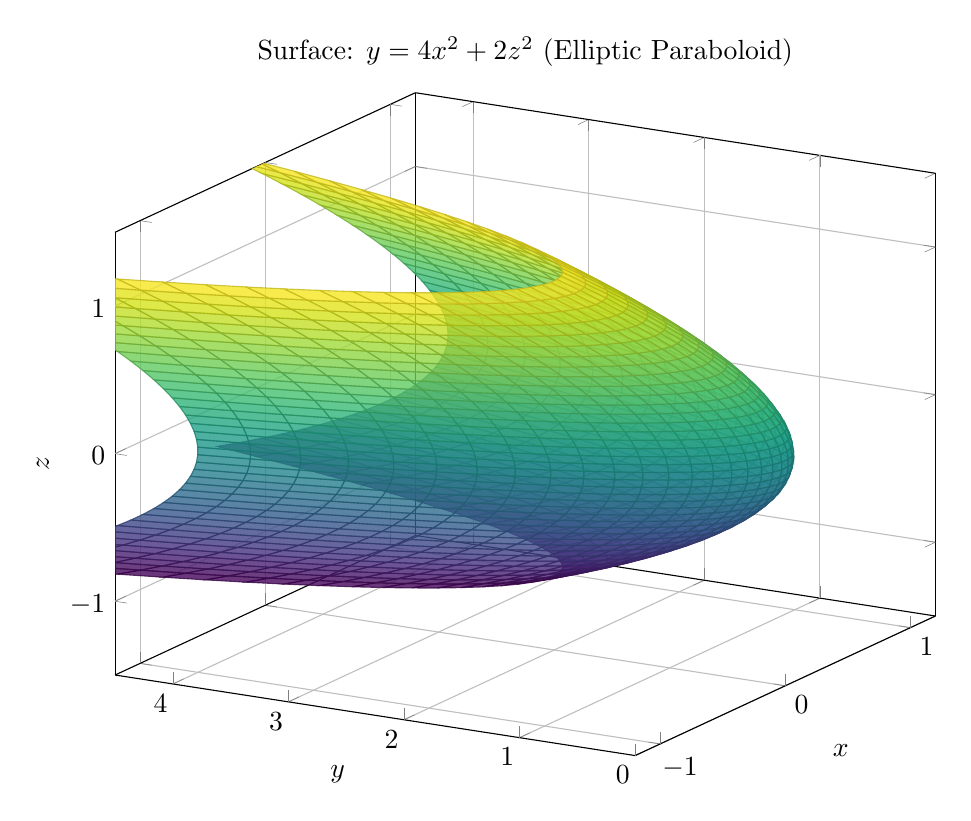
\begin{tikzpicture}
\begin{axis}[
    width=12cm,
    height=10cm,
    xlabel=$x$,
    ylabel=$y$,
    zlabel=$z$,
    title={Surface: $y = 4x^2 + 2z^2$ (Elliptic Paraboloid)},
    view={-60}{20},
    colormap/viridis,
    grid=major,
    zmin=-1.5,
    zmax=1.5,
    xmin=-1.2,
    xmax=1.2,
    ymin=0,
    ymax=4.5,
]
\addplot3[
    surf,
    domain=-1:1,
    y domain=-1:1,
    samples=40,
    samples y=40,
    opacity=0.8,
] ({x}, {4*x^2 + 2*y^2}, {y});
\end{axis}
\end{tikzpicture}
\end{document}